\documentclass[a4paper,12pt,oneside]{article}
%Chargement des packages
\usepackage[utf8]{inputenc} % l'encodage des fichiers est utf-8, mettre [latin1] si necessaire
\usepackage[english, portuguese]{babel}

%\usepackage[headheight=30pt,showframe]{geometry}
\usepackage[headheight=30pt]{geometry}

\usepackage{amsmath,amsfonts,amssymb,amsthm}

\usepackage{graphicx} %pour afficher des images
\usepackage{float}	%pour forcer le placement des images.

\usepackage{fancyhdr} %pour modification des pieds de page

\usepackage[usenames,dvipsnames]{color} % pour les textes en gris

\usepackage{framed}


\usepackage{hyperref} %pour que les références soient des liens hypertextes
%\hypersetup{
%    colorlinks=true,
%    linkcolor=blue,
%    filecolor=magenta,      
%    urlcolor=cyan,
%}

% package used by \citep and \citet
\usepackage[sort&compress,round,authoryear]{natbib}

%\renewcommand*\rmdefault{ptm}
%\renewcommand*\rmdefault{ppl}

\theoremstyle{plain}
\newtheorem{thm}{Teorema}[section]
\newtheorem{lem}[thm]{Lemma}
\newtheorem{prop}[thm]{Proposition}
\newtheorem*{cor}{Corollary}

\theoremstyle{definition}
\newtheorem{defn}{Definição}[section]
\newtheorem{conj}{Conjecture}[section]
\newtheorem{exmp}{Example}[section]

\theoremstyle{remark}
\newtheorem*{rem}{Remark}
\newtheorem*{note}{Note}

\usepackage{natbib}

% Comment utiliser : 
% - la page de titre est à personnaliser (title/title.tex)
% - le contenu est à rédiger dans le répertoire pages/, s'inspirer des exemples présents dans ce modèle.
% - les annexes sont à rédiger dans le répertoire appendix/
% - la bibliographie utilise BibTex (fichier biblio.bib)
% - les variables suivantes sont à remplir :
\newcommand{\TitreRapport}{Uma Introdução à Lingüística Computacional}
\newcommand{\DateRapport}{2017}
\newcommand{\AuteurRapport}{Gabriel Stefanini Vicente}
\newcommand{\NomEntreprise}{Universidade Estadual de Campinas}


%définition des marges
\geometry{hmargin=2.5cm, vmargin=2.5cm } 

%utilisation des puces anglaises.
%attention, il faut avoir une version récente de frenchb.ldf. 
%\frenchbsetup{StandardItemLabels}

%Définition des en-têtes et pieds de page
\renewcommand{\headrulewidth}{2pt}
\renewcommand{\footrulewidth}{0pt}

\fancyhead[C]{{}}
\fancyhead[RE, LO]{
\includegraphics[width=1cm]{style/images/logo-unicamp-anon-line-blk-blk-0120.png}}
\fancyhead[R]{{}} 

%\fancyfoot[C]{\textcolor{Gray}{\small\TitreRapport}}
\fancyfoot[C]{{}}
%\fancyfoot[RE, LO]{
\includegraphics[width=1cm]{style/images/logo-unicamp-anon-line-blk-blk-0120.png}}
\fancyfoot[LE, RO]{\thepage}

% définition du tire, de la date et de l'auteur du document
\title{\TitreRapport}
%\date{\DateRapport}
%\author{\AuteurRapport}
\setlength{\parindent}{1cm}

\renewcommand\maketitle{
\begin{titlepage}

\begin{center}
 	
\includegraphics[scale=0.25]{title/images/PRETO.JPG}
 	\hspace{\stretch{0.5}}
 	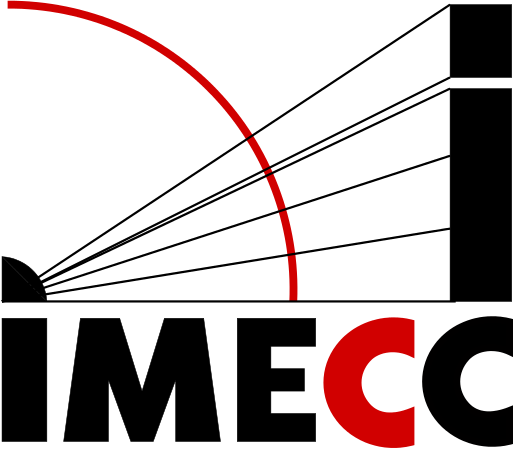
\includegraphics[scale=0.1]{title/images/logo-imecc.png}
 	\vskip 0.5cm
	\textit{\large{Universidade Estadual de Campinas
		\\ Instituto de Matemática, Estatística e Computação Científica}}
	\vskip 8cm      
    \textsc{\LARGE{\TitreRapport}}										
	\vskip 2cm    
	\textbf{\large{\\ \href{http://g4brielvs.me/}{\AuteurRapport} \\ \textit{\normalsize{IMECC - UNICAMP}}}} 
	\vskip 1cm
	\textbf{\large{Orientador \\ \href{http://www.pablofaria.com.br}{Prof. Dr. Pablo Faria} \\ \textit{\normalsize{IEL - UNICAMP}}}}
	\vskip 4cm
    \normalsize{Campinas, \today}
\end{center}    
\newpage

\begin{center}
\vspace*{16cm}
\begin{framed}
Escrito com a distribuição \TeX Live 2016
\end{framed}

\begin{framed}
\textbf{Aviso} ---   Esta obra é licenciada sob os termos da \emph{Licença
Creative Commons Atribuição-Não-Comercial-Compartilha-Igual 3.0 Brasil}. Para
qualquer reutilização ou distribuição, você deve deixar claro a terceiros os termos
da licença a que se encontra submetida esta obra. A melhor maneira de fazer isso é com um link para a página 
\url{https://creativecommons.org/licenses/by-nc-sa/3.0/br/}.

\vskip 0.5cm
\centering
	    
\includegraphics[width=4cm]{title/images/cc-nc-sa.png}
\end{framed}

\end{center}   
\end{titlepage}
\setcounter{footnote}{0}}

\makeatother


\begin{document}
\pagestyle{fancy}
\maketitle

\section*{Agradecimentos}

Em reconhecimento das discussões, ideias e correções, eu gostaria de expressar minha gratidão ao Prof. Dr. Pablo Faria pela orientação ao longo dos estudos dirigidos, sobretudo, pelas boas vindas a um forasteiro curioso pela Lingüística.
\newpage

\selectlanguage{portuguese}
\begin{abstract}

A capacidade de linguagem é uma das maiores vantagens evolutivas dos seres humanos. Comunicação verbal e escrita são a maneira fundamental pela qual é possível passar informação e conhecimento para novas gerações e resolver problemas abstratos e complexos em uma sociedade. Apesar de crianças começarem a falar com grande naturalidade, ainda há muito a se entender sobre a aquisição de linguagem e o tema ocupa um papel central na pesquisa científica na Lingüística. Esse relatório tem o objetivo de introduzir a Aquisição da Linguagem do ponto de vista da Gramática Generativa. Em primeiro momento, é apresentado um breve do contexto histórico e, em seguida, é introduzido um breve \emph{framework} teórico. Em segundo momento, são mostrados pontos positivos e negativos de abordagens computacionais para a Aquisição da Linguagem.

\end{abstract}

{\bf Keywords: Lingüística Computacional, Aquisição de Linguagem}

\newpage

\selectlanguage{english}
\begin{abstract}

The capacity for language is one of mankind's most important evolutionary advantages. Verbal and written communication 
is the key to our ability to pass information and knowledge forward to younger generations and our capacity to address abstract and complex problems as a society. Even tough a child can easily start talking, language acquisition remains an intricate subject and is at the heart of scientific inquiry and intellectual curiosity in Linguistics. This report is an introduction to the study of Language Acquisition in the perspective of generative grammar. At first, it introduces the reader to a quick historical background and brief theoretical framework. At second, it summarizes positives and negatives perspectives about a computational approach to Language Acquisition.

\end{abstract}

{\bf Keywords: Computational Linguistics, Language Acquisition}

\newpage

\newpage

\tableofcontents
%\listoffigures
%\listoftables
\newpage

\section*{Introdução}
\addcontentsline{toc}{section}{Introdução}
\noindent
Quando se aborda com ingenuidade a aquisição de fluência de uma língua, o primeiro pensamento que ocorre é que esse processo seja supostamente trivial. Aliás, crianças na mais tenra idade o fazem com grande facilidade. Porém, qualquer curioso que se debruce sobre o problema será confrontado com percalços e paradoxos, desde o que significa a rigor aprender uma língua e, antes de tudo, a definição do que é uma língua.

Os estudos dirigidos tiveram o objetivo de introduzir o grande \emph{framework} teórico por trás da Aquisição de Linguagem. Em primeiro lugar, com intuito de contextualizar historicamente, é apresentado um resumo de como as teorias evoluíram de especulações filosóficas para um formato científico. A questão da origem da fala sempre permeou o imaginário mítico, comumente sendo considerada uma dádiva divina, teve historicamente uma aproximação maior com questões filosóficas que científicas e só ganhou o patamar de exploração científica com os esforços durante as mudanças do florescer das Ciências nos séculos XVIII e XIX.

Em seguida, é explorado o problema de aquisição de linguagem de um ponto de vista da Lingüística. Nesse segmento, são definidos os conceitos de competência e performance lingüísticas, quais seriam as qualidades necessárias para adquirir uma língua e a caracterização como processo biológico.

Por fim, são introduzidos os principais argumentos que sustentam a abordagem da aquisição de linguagem com base na Teoria de Aprendizagem e Gramática Generativa. Finalmente indicamos de que maneira abordagens computacionais têm a contribuir para atacar a solução do problema, mostrando diferentes pontos positivos e negativos. São discutivos os modelos generativo, estatístico, social e espacial e desenvolvimentista.
\newpage

\section{Da Filosofia à Linguística}

Lingüística é a Ciência por trás da compreensão da forma e estrutura das línguas humanas. Não há quem não tenha curiosidade 
pelo que é falado. É um fenômeno que nos parece tão natural e simples, mas quando se reflete sobre ela o que se encontra é uma complexidade que fascina qualquer cientista ou curioso. Talvez por essa razão a questão da origem da fala tenha permeado tão constantemente o imaginário mítico. É curioso que muitos mitos coincidem ao dizer que a linguagem é uma dávida divina. A capacidade de se comunicar abstratamente também é um importante fator nos distingue de todos outros seres vivos que habitam o planeta: capacidade de aprender e ensinar através da língua. 

Nessa primeira seção, será tratado o percurso que levou o estudo das línguas evoluir de uma esfera de especulação do pensamento filosófico para um exercício científico. Muito foi descoberto a respeito da natureza dos processos cognitivos, isto é, se era uma discussão reservada para a abstração, experimentações passaram a mostrar como mensurar fenômenos da mente.

\subsection{Filosofia da Mente}

O problema Mente-Cérebro é a dicotomia entre mundo interior e o mundo físico na experiência da consciência. Existem evidências antropológicas que sustentam a crença de que os primeiros seres humanos já tinham o entendimento da diferença entre corpo e alma. Para os filósofos da Antigüidade, era de conhecimento geral ser o cérebro o órgão responsável pelos sentimentos, sentidos e inteligência. No Renascimento, com o florescer das Ciências Naturais, muito foi descoberto nas áreas de Anatomia e Fisiologia. Porém, a questão da origem e manifestação da consciência ainda estava em aberto. 
Uma das primeiras grandes influências modernas para responder ao problema foi de René Descartes. Sua teoria propunha a existência de uma componente imaterial, chamada de \emph{res cogitans}, em oposição a uma componente material chamada de \emph{res extensa}. Esses dois componentes teriam papéis iguais para construção da consciência e interagiriam entre si no interior de estruturas cerebrais. Essa corrente ficou conhecida por Dualismo. Graças a essa forma de pensar, pouco a pouco o estudo da mente começou a ganhar o domínio mais exato nos campos da Fisiologia e Medicina. Esse avanço deu nascimento à Psicologia Experimental.

\subsection{Psicologia Experimental}

Diante do florescer das Ciências Naturais na Revolução Científica durante os séculos XVII  XVIII, grandes cientistas contribuíram para o entendimento da mente pelo viés empírico e epistemológico. Graças à invenção do microscópio e descobertas no estudo de anatomia humana, os conhecimentos sobre o sistema nervoso foram consolidados e exploradas suas relações com outros sistemas do corpo. 

No século XIX, Hermann Helmholtz foi responsável em calcular a velocidade da condução nervosa. Esse resultado teve uma forte influência para Psicologia Científica ao constatar que a comunicação através de nervos não é instantânea e ocorre via excitação elétrica. Porém, somente anos mais tarde que vieram as bases do que hoje é chamada Psicologia.

De um ponto de vista quantitativo, o primeiro cientista a se dedicar a estudos psicológicos foi o alemão Ernst Weber. No início do século XIX, seu interesse acadêmico o pôs a explorar a fisiologia por trás da resposta a estímulos externos, sobretudo, envolvendo a sensação de tato. Foi o responsável por realizar os primeiros estudos de limiares. Sua contribuição principal foi na percepção de pressão sobre a pele. Ele propôs um experimento para avaliar em que momento é percebida uma diferença de pressão. Em teste cego, voluntários comparam um peso padrão com pesos de teste, pedindo-se para discriminar o mais leve ou o mais pesado.  A conclusão, conhecida por Lei de Weber, é de que não se percebe a diferença entre os objetos, mas a proporção dessa diferença com a magnitude dos objetos. Portanto, a lei de Weber expressa a diferença necessária para perceber o estímulo como diferente. 

Em seguida, Gustav Fechner, tendo ciência dos trabalhos de Weber, aprimorou o método dos limiares e estudo de percepções. No seu entendimento, as diferenças refletiam não somente uma diferença quantitativa, mas uma diferença psicológica. Em outras palavras, a percepção de estímulo, mesmo podendo ser mensurado, tem inerentemente um caráter subjetivo. Fechner também foi responsável por executar experimentos com estímulos visuais e sonoros, chegando a conclusões semelhantes.
Por sua vez, coube ao alemão Wilhelm Wundt a formalização desses esforços na forma de uma nova ciência. Sendo fundador do primeiro laboratório de Psicologia, foi o pioneiro em experimentação com a mente e a consciência. Wundt estabeleceu a distinção entre psicologia experimental, sujeita a métodos científicos mais tradicionais e trabalhos de laboratório, e psicologia cultural, que caberia a um escopo mais filosófico. Além disso, criou uma metodologia clara fazendo a distinção de faculdades elementares, passíveis de reprodução em laboratório, e faculdades superiores, tais como linguagem. Para Wundt, a consciência não se trata de moralidade, mas de uma consciência perceptual. Wundt foi um dos pesquisadores mais produtivos, escrevendo, em média, três páginas por dia ao longo de sua vida.

O cientista James Cattell foi o primeiro americano a receber o título de doutor sob a orientação de Wundt. Muito influenciado pela metodologia das escolas alemãs, Cattell foi o principal incubido de desenvolver e concretizar a visão de Wundt. Cattell realizou experimentos para obter tempo de resposta introduzindo complexidade nas tarefas. Por exemplo, em um de seus ensaios, na primeira etapa pede-se a um voluntário que somente indique quando perceber o acendimento de um sinal luminoso. Na segunda etapa, pede-se que indique somente quando o sinal for de uma determinada cor. A diferença de tempo deve representar o tempo de processamento no cérebro.  Assim, o cientista coletou as primeiras medidas mais assertivas de cronometria mental. Cattell foi um pioneiro em experimentos envolvendo linguagem. 

Nesse contexto, a linguagem passou a ser estudado como um processo cognitivo como qualquer outro, passível de experimentação.

\subsection{Teoria Cognitivista}

No início do século XX, a Psicologia foi fortemente influenciada pelos trabalhos Skinner e outros cientistas behavioristas. Nessa corrente científica, colocava-se como objeto de estudo o comportamento. Para Skinner, a mente tem uma natureza intangível e não-observável, cabendo então à pesquisa científica somente estudar o comportamento. Esse período ficou conhecimento como a fase em que "Psicologia perdeu a cabeça". Os resultados relacionados a condicionamento de comportamento e aprendizado tiveram grande influências nos métodos militares e escolares usados até hoje em dia. Muito também foi descoberto a respeito do comportamento animal e quão semelhante é comparado ao ser humano.

Entretando, anos mais tarde nos anos 1950, esforços de diferentes áreas, desde Ciência da Computação até Psicologia, argumentavam que essa abordagem não seria suficiente para explicar todos fenômenos cognitivos. O principal argumento era que o modo de pensar seria instrinsecamente um processo da mente e afetaria o comportamento, sendo assim, inadequado se limitar ao estudo da conseqüência, isto é, do comportamento por si só. Esse período ficou conhecido por Movimento Cognitivista. Apesar de trazer de volta para o holofote o estudo a mente, a abordagem cognitivista faz fortemente uso de métodos quantitativos, buscando descrever as funções da mente e o processamento das informações. Particularmente na Lingüística, houve uma grande contribuição para nascimento da Gramática Generativa. O linguista norte-americano Noam Chomsky \citep{chomsky65} propôs a capacidade da linguagem pode ser vista como uma gramática constituída por um sistema de regras para combinação de palavras e formação de sentenças. Nesse contexto, adquirir uma linguagem equivale a ganhar domínio sobre esse sistema de regras.







\newpage

\section{Aquisição de Linguagem}

A Aquisição da Linguagem é para muitos um dos problemas centrais da Lingüística. Porém, o estudo dos processos relacionados à capacidade de linguagem e inteligência não são exclusivos aos lingüistas. Como já mencionado, a origem das línguas sempre permeou a imaginação coletiva, sendo um frutífero campo para ficção e filosofia. Além disso, a habilidade de falar e conceber e comunicar ideais é compreendida como um grande indicativo de consciência. Curiosamente, as primeiras tentativas na direção do estabecimento mais formal do estudo da linguagem vêm dos esforços da Matemática e Inteligência Artificial. O matemático Alan Turing \citep{turing1950computing} já levantava a questão se máquinas seriam capazes de pensar. Turing sugeriu trocar as palavras \emph{pensar} e \emph{máquina} por um critério mais claro e concreto. A ideia era testar se uma máquina é capaz de demonstrar comportamento inteligente. Hoje é conhecido como Teste de Turing. Analogamente, na área da Teoria  da Aprendizagem, busca-se definir com rigor matemático o que significa adquirir a capacidade de linguagem ou, em outras palavras, adquirir e dominar competências lingüísticas. Logo, no presente contexto, a aquisição de linguagem será vista como processos cognitivos e lingüísticos que permitem o falante de se expressar em uma língua, tendo como base a teoria da Gramática Generativa.

\subsection{Competência Lingüística}

Um falante nativo é capaz de avaliar se frases fogem a uma regra de sua língua ainda que não saiba a razão específica da suspeita. Hipoteticamente, se lhe fosse pedido registrar todo seu conhecimento, dar-se-ia conta de não ter todo conteúdo em nível consciente, apesar de ser capaz de se comunicar fluentemente. Essa habilidade intrínseca e inconsciente é sua competência na língua. Já sua real capacidade de articular e por em prática uma linguagem é chamada de performance.
 A distinção entre as duas é bem nítida para qualquer falante, uma vez que é comum se atrapalhar para construir frases, parar no meio e reformular, errar conjugação de um verbo e não é por isso que não se assume conhecimento lingüístico. Essa distinção é um importante marco teórico \citep{chomsky65} para salientar a diferença entre não ter conhecimento pleno e somente cometer um deslize de fala na produção da língua. \\
 
Em suma, falar uma língua implica ter o domínio de diferentes níveis lingüísticos, isto é, 
ter a habilidade de usar diferentes qualidades relacionadas à linguagem. No quadro abaixo está sumarizado o conjunto dessas qualidades e suas respectivas áreas de estudo dentro da Lingüística.
 
\begin{center}
\begin{tabular}{| l | l | l |}
 \hline 
 \textbf{Constituintes} &  \textbf{Capacidade} & \textbf{Área} \\ 
 \hline 
 Sons & Fonemas & Fonética/Fonologia \\ 
 \hline 
 Palavras & Léxico & Morfologia \\ 
 \hline 
 Sentenças & Combinação de palavras & Sintaxe \\ 
 \hline 
 Conceitos & Sentido das senteças & Semântica \\ 
 \hline 
 Intenções & Propósito da fala & Pragmática \\ 
 \hline 
 \end{tabular}  
 \end{center}
 
Na investigação lingüística, mais particularmente na Aquisição de Linguagem, o que se propõe é elucidar como cada qualidade está relacionada ao processo de aquisição de linguagem e construção da gramática do falante. Abaixo, temos questões que cada área da Lingüística deveria ser capaz responder ao passo que um falante o faz natural e inconscientemente. \\
 
 \begin{itemize}
 \item Fonética
 	 \begin{itemize}
 		\item Quais são os sons elementares de uma linguagem?
 		\item Como segmentar e combinar sons em palavras?
 	\end{itemize}
 \end{itemize}

\begin{itemize}
 \item Morfologia
 	 \begin{itemize}
		\item Quais são as unidades de sentido (palavras)?
		\item Como identificar segmentação entre palavras na fala?
		\item Como identificar a quais pessoas, objetos ou eventos as palavras se referem?
		\item Como construir vocabulário funcional?
 	\end{itemize}
 \end{itemize}
 
 \begin{itemize}
 \item Sintaxe
 	 \begin{itemize}
		\item Como combinar palavras para construir sentenças que carregam sentido?
		\item Qual é a hierarquia de palavras de uma sentença?
		\item Como classificar uma sentença como gramatical?
 	\end{itemize}
 \end{itemize}

 \begin{itemize}
 \item Pragmática
 	 \begin{itemize}
		\item Como demonstrar intenção?
 	\end{itemize}
 \end{itemize}

\subsection{Processo Biológico}
\label{sec:processobiologico}

A aquisição de linguagem antes de tudo é tida como um processo biológico, similar de outros órgãos do corpo, pela perspectiva chomskiana. Uma série de evidências reforçam a proposição de se tratar de um processo biológico, valendo destacar:

\begin{itemize} 
\item Progressão de estágios \\
Em analogia a outros fenômenos biológicos, como reprodução ou ganhar habilidade de voar, a aquisição também evolui em seqüência. Por exemplo, produzir sons vem antes produzir palavras; produzir palavras antes de sentenças.  
\item Linha do tempo comum \\
Outra evidência é que diferentes crianças adquirem capacidades lingüísticas na mesma posição aproximada no tempo.
\item Período crítico \\
É observável que existe um período depois do qual a aquisição de linguagem se torna prejudicada. Crianças demonstram menos facilidade de aquisição de uma segunda língua após a primeira infância. Há inclusive casos extremos de privação total, em que se torna impossível adquirir fluência na língua pelo indivíduo, mesmo quando exposto mais tardiamente à linguagem. Essas observações sustentam a hipótese de que durante a primeira infância existem componentes biológicos em ação que são suprimidos no decorrer da vida.
\item Independência de estímulo externo \\
Observar que crianças surdas são capazes de produzir sons e se comunicar leva a crer que a linguagem é uma decorrência de um programa biológico e não exclusivamente dependente de estímulo externo. Vale lembrar que como outros fenômenos da natureza, é preciso estímulo para que se desenvolva por completo, por exemplo, sem uma nutrição mínima, o organismo não se desenvolve corretamente e até mesmo pode morrer. 

\end{itemize}

Se postos lado a lado, um bêbe humamo e um chimpanzé, assusta-se perceber que o segundo vai nos superar em muitas tarefas. Sobretudo, em se tratando de memorização. Incrivelmente, um ser humando, poucos anos depois, é capaz de dominar grande número de sentenças e conceitos. Os seres humanos parecem ter um instinto para linguagem como pássaros têm para voar e formigas para sociedade \citep{pinker94}.

\subsection{Teoria de Aprendizagem}

Aquisição da Linguagem é o processo pelo qual seres humanos tornam-se capazes de compreender e reproduzir uma língua. Esse processo, de um ponto de vista analítico, pode ser abordado a partir de questões de \emph{o quê}, \emph{quando} e \emph{como} um indivíduo desenvolve uma determinada habilidade lingüística \citep{pearl2010}. Então, seria possível organizar, de maneira simplificada, um fluxo lógico dos processos que levariam à aquisição de uma língua nas perguntas abaixo.

\begin{itemize}
\item Qual é o objeto a ser aprendido?
\item Quando o objeto é aprendido?
\item Como o objeto é aprendido?
\end{itemize}

Pensando na língua mãe, o objeto em questão são competências e conhecimento lingüísticos que a criança adquire, isto é, as palavras e os fonemas e, junto com eles, a carga semântica e regras sintáticas. O próximo passo é analisar o momento em que cada habilidade é dominada e estabelecer uma seqüência ordenada de acontecimentos, pontuando na linha do tempo marcas de proficiência com a língua. Por exemplo, a capacidade de discernir palavras na fala é obviamente anterior à capacidade de conjugar verbos no passado.

Contudo, analisar exatamente o desenrolar dessa etapas, isto é, \emph{como} a criança aprende \emph{o que} até o tempo de \emph{quando}, é mais intrincado. De todas as perguntas, o \emph{quando} é o mais bem resolvido, talvez por se tratar da parte mais empírica e observável das três. Se expostas a estímulos lingüísticos, crianças adquirem domínio sobre habilidades na linguagem em torno da mesma faixa de idade e com um conjunto similar de vocabulário. Além disso, o processo de aquisição se dá em etapas sucessivas e facilmente reconhecidas, como mencionado na seção \ref{sec:processobiologico}. Por exemplo, a identificação dos sons é anterior à combinação de palavras e a fala é anterior à escrita \citep{bertolo2001language}.

Agora a questão de \emph{o que}, isto é, o conhecimento lingüístico adquirido ganha um grau de complexidade maior. Como veremos na seção a seguir, não é possível que um indivídio seja exposto a todo conteúdo de uma língua, porém, toda criança é capaz de generalizar e aprender as regras da linguagem e passar a formar suas próprias sentenças. Existe grande esforço acadêmico nessa investigação, tanto por sua natureza científica quanto pela natureza prática e comercial devido ao uso que se pode ter em aplicacões.

A questão do \emph{como}, por fim, talvez seja a mais filosoficamente interessante e a mais resistente a métodos quantitativos. A capacidade de linguagem é uma característica absolutamente humana, o que leva a crer que deve existir alguma estrutura biológica exclusiva, visto que o cérebro humano não difere muito de tamanho de outros animais, inclusive proporcionalmente.

\subsubsection{Estímulo Positivo e Estímulo Negativo}

Todo estímulo lingüístico pode ser classificado como positivo ou negativo no sentido de ser uma forma válida ou não-válida dentro da língua em questão, isto é, se é gramatical ou agramatical. Uma criança exposta à fala de adultos é submetida a estímulos positivos na maior parte do tempo. Se recebe estímulos negativos, nunca é apresentada com explicações ou categorizações. Contudo, a criança é capaz de extrapolar a experiência e passar a formular suas próprias sentenças. Outro ponto é quando criança chega a inferir regras incorretas, ela muitas vezes não é corrigida, não tendo estímulos negativos. Apesar da falta de evidências negativas, a criança é capaz de evitar e eliminar erros de sua fala e consegue reproduzir a gramática de sua língua com o tempo.
A limitação de estímulo, tanto da insuficiência de evidência positiva quanto da falta de evidência negativa, deu origem ao argumento da  \emph{pobreza de estímulos} (do inglês, \textit{poverty of stimulus}). Esse é um argumento importante para a hipótese de que desenvolver um sistema complexo como a gramática de um adulto a partir de um conjunto limitado de informações deve pressupor uma capacidade inata para linguagem \citep{chomsky65}.

\subsubsection{Gramática Universal}

Em resposta ao argumento anterior, Chomsky propõe a Gramática Universal \citep{chomsky65}. Um falante é capaz de compreender e produzir um número aparentemente infinito de expressões lingüísticas, apesar do conjunto limitado de estímulos positivos e negativos ao qual é exposto. Não é possível pensar em um modelo indutivo que resolva esse paradoxo, o que leva a hipótese de uma dotação inata que permitiria a capacidade de uma atividade complexa como a linguagem.

\section{Lingüística Computacional}

Ao se atacar o problema de aquisição de linguagem, existem muitas formas de abordagem. O uso de ferramentas computacionais e modelos matemáticos contribuíram para a evolução desde sua introdução pelos cognitivistas. O principal benefício de uma abordagem computacional é que se trata de uma simulação, assim sendo possível ter controle e flexibilidade sobre as condições que se deseja experimentar \citep{frank2011}.

Ao se reproduzir o comportamento do ser humano em uma esquematizaçao ou em um computador, é importante esclarecer que não se faz necessário ter compreensão de todos processos em andamento. Segundo \citet{marr1982vision}, qualquer processo cognitivo pode ser dividido em três componentes:

\begin{itemize}
\item Computacional
\item Algorítmico
\item Implementacional
\end{itemize}

Na etapa computacional, tem-se o interesse de descrever o problema em questão, suas premissas e condições. Na etapa algorítmica, o centro da pesquisa é o modo como os processos de desenrolam. Por último, na etapa implementacional, tem-se um realização concreta do experimento. É nesse item que simulações computacionais trazem muitas contribuições, graças à possibilidade de controlar as entradas e saídas.

Ainda dentro de uma abordagem computacional, existem muitas vertentes com preposições, abordagens e modelos diferentes\citep{kaplan:inria-00348493}. A seguir, algumas serão apresentadas.

\begin{itemize}
\item Generativa \\
Essa é a visão que mais dominou o estudo da área desde o surgimento. Segundo ela, a aquisição de linguagem consiste no aprendizado da sintaxe, isto é, a função de classificar sentenças em gramaticais e agramaticais. Computacionalmente, o objetivo é de mapear um espaço de sentenças $S$ nas respostas \emph{gramatical} ou \emph{agramatical}. Esse é um problema muito parecido com aprendizado estatístico ou de máquina, em que existe um espaço de exemplos para treinamento e uma classificação no final. O que difere essa abordagem fortemente de um problema de classificação usual é a hipótese de pobreza de estímulos, ou \textit{poverty of stimulus}, segundo a qual nunca seria possível construir um modelo completo da gramática considerando-se a limitação dos estímulos. Nesse ponto de vista, o interesse maior está em construir a competência lingüística a partir de amostras.

\item Estatística \\
A hipótese de pobreza de estímulos, ou \textit{poverty of stimulus}, foi colocada em questão em experimentos mostrando ser possível extrair padrões lingüísticos de sons e sentenças. Em contraste com o item anterior, o interesse maior está em modelar a performance lingüística. Essa abordagem é a mais aberta para as técnicas estatatísticas e de aprendizado de máquina, fazendo um algoritmo capaz de avaliar sentença um problema de classificação por excelência. Como principal desvantagem está que só é possível aprender estruturas com grande ocorrência na língua. Também se faz necessário o uso de grandes \emph{corpora} para que os resultados tenham relevância. De qualquer modo, é uma das principais abordagens adotadas por programadores quando se trata de problemas envolvendo linguagens naturais.

\item Socia e Espacial \\
É importante ressaltar que muitos modelos matemáticos e computacional ignoram a componente social na aquisição de linguagem. Contudo, é claro que tanto o aprendizado quanto a expressão de uma língua têm forte peso da sociedade e meio em que se está inserido. Essas abordagens têm grande contribuição para o entedimento do contexto e semântica da fala. Por exemplo, se durante um processo de aprendizado de máquina existir um contexto de ação, é muito mais fácil fazer inferências e diminuir ambigüidades.

\item Desenvolvimentista \\
As abordagens anteriores descrevem o processo de aprendizado como contínuo e determinístico, em que o falante tem pouco poder de ação, isto é, o indíviduo seria somente exposto a estímulo de outros indíviduos ou do ambiente e passaria a adquirir graças a uma faculdade inata. Alguns linguistas acreditam que a aquisição de linguagem também se deve a maneira de explorar o conhecimento lingüístico de uma forma não-linear e não-determinística. Para eles, todo processo é desenvolvido progressivamente ao se interagir e com o modo de se interagir com outras pessoas e outras ideias.

\end{itemize}

\subsection{Abordagem com aprendizado de máquina}

Em 1997, um ser humano foi vencido por um computador em uma partida de xadrez\footnote{\url{http://www-03.ibm.com/ibm/history/ibm100/us/en/icons/deepblue/}}. O super computador Deep Blue superou somente com circuitos e algoritmos um dos limites de inteligência humana. Porém, vale lembrar que foram necessários mais de cinqüenta anos de pesquisa, engenho e sorte. Mas, no final, uma máquina superou o ser humano. Em 2017, Google realizava testes com um veículo autônomo\footnote{\url{http://www.google.com/selfdrivingcar/}}, isto é, sem a necessidade de um motorista humano. Novamente, fomos vencidos.

Agora, basta ter uma conversa com a Siri ou a Alexa para perceber que ninguém jamais aceitaria um convite para jantar de qualquer uma delas. Embora rendam boas piadas, os seus mecanismos de fala são muitos artificiais. O que torna a capacidade de falar tão inerentemente humana? E o que torna falar tão intricamente difícil? Aliás, uma criança de 5 anos é capaz de falar com naturalidade, apesar de não fazer ideia do que fazer com uma alavanca do câmbio de marchas.

Embora as técnicas de Inteligência Artificial tenham evoluído muito e novas capacidades computacionais tenham surgido, a linguagem ainda tem um grau de complexidade resistente a uma apreensão plena pelos métodos da área. A maioria das soluções de aprendizado de máquina fazem uso de propriedades estatísticas nas massas de dados e extrapolam padrões. Porém, tudo indica que a linguagem não é uma mera repetição de padrões e que deve existir um instinto ou uma habilidade inata para adquirir uma língua.

De qualquer modo, já existem muitos exemplos de aplicações com linguagens naturais usando-se técnicas estatísticas, como corretores de texto, transcrições automáticas de fala e tradutores.
\newpage
\section*{Comentários Finais}
\addcontentsline{toc}{section}{Comentários Finais}

O estudo da aquisição de linguagem mostrou-se um campo frutífero e intersdisciplinar. A linguagem sempre suscitou a curiosidade filosófica e científica, tendo seu entendimento um longo histórico e com grande evolução até o presente momento. Desde do estabelecimento como uma ciência, a Lingüística e, mais particularmente a Aquisição da Linguagem, ganhou técnicas e métodos para pesquisa e análise. Os experimentos precursores durante os séculos XVIII e XIX deram a base para a formalização das teorias cognitivistas. Durante o século XX, o mundo assistiu um movimento a caminho da estruturação das Ciências Humanas e, em conseqüência, os lingüistas receberam contribuições de outras disciplinas e de outras teorias.

A partir desse momento, a Teoria de Aprendizagem e Inteligência Computacional muniram o estudo da aquisição de linguagem de métodos quantitativos e matemáticos. Essa união teve resultados produtivos. Primeiramente, ao se criar uma representação de um fenômeno lingúístico, é preciso ter consciência das variáveis livres e dependentes e quais são as suas relações, o que contribui para o entendimento do problema como um todo. Além disso,  usando uma simulação computacional, é possível testar e levantar hipóteses com grande facilidade, não se limitando a condições físicas ou sociais. É importante lembrar que a Ciência da Computação e Lingüística se complementam em uma via de mão dupla. Da mesma maneira que máquinas auxiliem no estudo da linguagem, as teorias lingüísticas dão a base para a existência de inúmeras aplicações, por exemplo, correções de texto, traduções e transcrições.
\newpage

\bibliographystyle{apalike}
\bibliography{bibliography} 
\addcontentsline{toc}{section}{Referências}

%\appendix
%\input{appendix/titreA.tex}

\end{document}
